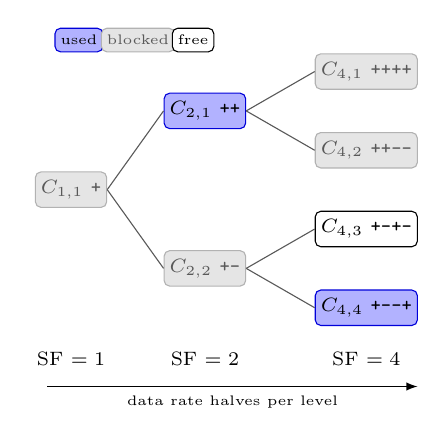
\begin{tikzpicture}[
    >=latex,
    code/.style={draw, rounded corners=2pt, font=\scriptsize, inner sep=2pt, minimum height=0.45cm},
    used/.style={code, fill=blue!30, draw=blue!85!black},
    blocked/.style={code, fill=gray!20, draw=gray!60, text=gray!70!black},
    free/.style={code, fill=white}
]
    % OVSF code tree: C(2n,2k-1) = [C(n,k), C(n,k)], C(2n,2k) = [C(n,k), -C(n,k)]
    \node[blocked] (c11) at (0,0) {$C_{1,1}$ \texttt{+}};

    \node[used] (c21) at (1.7,1.0) {$C_{2,1}$ \texttt{++}};
    \node[blocked] (c22) at (1.7,-1.0) {$C_{2,2}$ \texttt{+-}};

    \node[blocked] (c41) at (3.75,1.5) {$C_{4,1}$ \texttt{++++}};
    \node[blocked] (c42) at (3.75,0.5) {$C_{4,2}$ \texttt{++--}};
    \node[free] (c43) at (3.75,-0.5) {$C_{4,3}$ \texttt{+-+-}};
    \node[used] (c44) at (3.75,-1.5) {$C_{4,4}$ \texttt{+--+}};

    \foreach \a/\b in {c11/c21, c11/c22, c21/c41, c21/c42, c22/c43, c22/c44} {
        \draw[gray!70!black] (\a.east) -- (\b.west);
    }

    % Spreading factor per level
    \foreach \x/\sf in {0/1, 1.7/2, 3.75/4} {
        \node[font=\scriptsize] at (\x,-2.15) {SF $=\sf$};
    }
    \draw[->] (-0.3,-2.5) -- (4.4,-2.5) node[midway, below, font=\tiny] {data rate halves per level};

    % Legend
    \node[used, minimum height=0.3cm, font=\tiny] at (0.1,1.9) {used};
    \node[blocked, minimum height=0.3cm, font=\tiny] at (0.85,1.9) {blocked};
    \node[free, minimum height=0.3cm, font=\tiny] at (1.55,1.9) {free};
\end{tikzpicture}
